\chapter{Implementasi dan Pengujian}
\label{chap:implementation}
Pada bagian ini akan dijelaskan mengenai lingkungan implementasi perangkat keras maupun perangkat lunak. Serta implementasi program iCalendar Converter beserta tampilan antar muka. Terakhir akan dibahas mengenai pengujian pada perangkat lunak ini.

\section{Implementasi}
Pada bab ini akan dijabarkan mengenai lingkungan pengembangan perangkat lunak disertai dengan pengujian.

\subsection{Lingkungan Implementasi}
Dalam mengimplementasikan program terdapat dua lingkungan pendukung, yaitu lingkungan perangkat keras dan lingkungan perangkat lunak.
\subsubsection{Lingkungan Perangkat Keras}
Dalam mengembangkan perangkat ini, digunakan spesifikasi perangkat keras sebagai berikut:
\begin{itemize}
	\item \textit{Processor} : Intel Core i7 2.4 Ghz
	\item \textit{Memory} : 8 GB
	\item \textit{Hardisk} : 640 GB
	\item VGA : Nvidia GeForce 540M
	\item \textit{keyboard} dan \textit{mouse standard}
\end{itemize}

\subsubsection{Lingkungan Perangkat Lunak}
Untuk pengembangan perangkat lunak iCalendar Converter, digunakan spesifikasi sebagai berikut:
\begin{itemize}
	\item IDE : Netbeans 8.1
	\item JDK : 1.8
	\item JRE : Java Runtime Enviroment 8
	\item Serta library pihak ketiga seperti JavaFX, Apache POI, dan iCal4j
	\item Editor antarmuka menggunakan SceneBuilder
\end{itemize}

\subsection{Implementasi Program}
Subbab ini menjelaskan tahap dimana program akan dibuat dan dikembangkan dari hasil analisis dan perancangan kelas-kelas maupun \textit{method} yang digunakan. Kode program lengkap dapat dilihat pada Lampiran A. 
Berikut ini merupakan penjelasan kode program dari perangkat lunak iCalendarConverter :
\begin{enumerate}
	\item Kode Program untuk menyimpan jadwal \\
	ScheduleClass merupakan kelas model yang ditujukan untuk menyimpan informasi jadwal yang telah dibaca.\\
	Baris (115-127) kelas ScheduleClass pada lampiran ~\ref{lst:ScheduleClass} menjelaskan tentang penggunaan StringProperty 
	dimana sebuah property memungkin untuk memberitahu jika ada perubahan pada variable tersebut. Property membantu untuk menjaga tampilan agar singkron dengan data. Pada ScheduleClass variable yang menggunakan StringProperty adalah dosen, subject, dan location.	
	\item Kode program untuk membaca Excel \\
	ExcelConverter merupakan kelas yang dikhususkan untuk membaca excel dan mengeluarkan \textit{output} berupa Arraylist dari kelas model ScheduleClass.\\
	Berikut ini merupakan urutan dari algoritma yang digunakan pada Excel Converter :
\begin{enumerate}
		\item Baris (68-84) pada lampiran ~\ref{lst:ExcelConverter} menjelaskan bagaimana program mencari kolom No. dan Nama Mata Kuliah pada excel, sebagai acuan bahwa setelah kolom itu merupakan data jadwal yang akan dibaca oleh program. Setelah diketahui dimana kolom No. dan Nama Kuliah berada, nomer baris dan kolomnya akan dimasukan kedalam variable sebagai acuan membaca program dimulai pada baris itu. Pemilihan kolom No. sebagai acuan karena isi kolom No. menandakan berapa banyak data jadwal yang ada, sehingga bila isi dari kolom No. bukan angka maka program akan berhenti membaca. Selanjutnya, pemilihan Nama Mata Kuliah sebagai acuan selain karena data pada kolom itu akan dimasukan ke kelas model, pun juga karena setelah kolom tersebut terdapat kolom ruang kuliah yang akan dimasukan kedalam variable lokasi pada program.
		Selain itu, nomer kolom ruangan dapat menjadi acuan lokasi dosen mengawas.
		\item Baris (85-87) pada lampiran ~\ref{lst:ExcelConverter} menjelaskan bahwa i sebagai acuan program membaca baris, sedangkan j sebagai acuan program membaca kolom.
		\item Baris (89-93) pada lampiran ~\ref{lst:ExcelConverter} menjelaskan bahwa bila baris ke i program membaca dan isinya kosong maka berhenti membaca.
		\item Baris (96-100) pada lampiran ~\ref{lst:ExcelConverter} menjelaskan bila isi pada kolom No. bukanlah angka dan \textit{blank} maka program berhenti membaca.
		\item Baris (101-107) pada lampiran ~\ref{lst:ExcelConverter} menjelaskan	bila isi kolom No. adalah kosong maka lewati barisnya dan baca baris selanjutnya.
		\item Baris (108-129) pada lampiran ~\ref{lst:ExcelConverter} menjelaskan bahwa bila kolom tersebut tanggal maka, jika isinya kosong maka lewati barisnya, jika tidak kosong maka pisahkan isinya menurut tanda - dan tanda , . Lalu, jika ada singkatan Mrt ganti menjadi 3, jika ada singktan Okt ganti menjadi 10 dan jika ada singkatan 16 maka ganti menjadi 2016. Sehingga format tanggal menjadi 2016-03-01 sebagai contoh. Setelah itu masukan ke variable LocalDate.
		\item Baris (130-163) pada lampiran ~\ref{lst:ExcelConverter} menjelaskan bahwa bila kolom tersebut adalah jam maka, jika isinya LIBUR maka lewati baris tersebut, jika isinya Shift maka pasti baris dibawahnya adalah jam, sehingga ambil value baris dibawahnya lalu pisahkan menurut tanda - dan ganti tanda . dengan tanda : . Lalu, masukan ke variable LocalTime. Jika isi kolom berisi jam saja, maka pisahkan menurut tanda - dan ganti tanda . dengan tanda : . Lalu, masukan ke variable LocalTime.
		\item Baris (164-166) pada lampiran ~\ref{lst:ExcelConverter} menjelaskan bila kolom tersebut adalah Nama Mata Kuliah maka masukan ke variable String Subject.
		\item Baris (173-192) pada lampiran ~\ref{lst:ExcelConverter} menjelaskan bila kolom tersebut adalah ruangan yang bearti isinya adalah nama dosen yang mengawas maka, jika isi kolom diawali dengan Lab maka pisahkan menurut tanda : dan pisahkan kembali menurut tanda , sehingga menghasilkan nama dosen saja. Selanjutnya, masukan nama dosen ke ArrayList dosen dan isi ArrayList location dengan kata Lab. Jika isi kolom tidak di awali dengan kata lab maka masukan nama dosen ke ArrayList dosen dan isi ArrayList location dengan mengambil nomor kolom dari ruangan tersebut dan mencocokannya dengan posisi nama dosen tersebut berada dan isi nomer ruangan kedalam ArrayList Location.
		\item Baris (193-215) pada lampiran ~\ref{lst:ExcelConverter} menjelaskan bahwa karena dua mata kuliah berisikan dua baris kolom dosen yang di \textit{merger} jadi satu dan Apache POI hanya dapat membaca baris pertama kolom yang dimerger maka pada baris ini ArrayList dosen dan location disi dengan String kosong.
		\item Baris (219-221) pada lampiran ~\ref{lst:ExcelConverter} menjelaskan masukan semua variable yang diisi kedalam ArrayList ScheduleClass sesuai jumlah ArrayList nama dosen.
		\item Baris (222-223) pada lampiran ~\ref{lst:ExcelConverter} menjelaskan hapus semua isi ArrayList dosen agar tidak ada duplikasi.
		\item Baris (227) pada lampiran ~\ref{lst:ExcelConverter} menjelaskan hasil ArrayList method Converter() akan kembali dicek oleh method mergering().
		\item Baris (235-242) pada lampiran ~\ref{lst:ExcelConverter} menjelaskan jika ada dosen yang isinya kosong pada ArrayList ScheduleList maka pindahkan isinya ke ArrayList baru yang bernama ScheduleListSmt. Hal ini karena dua matakuliah yang berbeda di awas oleh satu dosen dan sehingga nantinya subject yang variable dosennya kosong akan dipindahkan ke variable dosen yang ada nama dosennya.
		\item Baris (243-250) pada lampiran ~\ref{lst:ExcelConverter} menjelaskan hapus isi ArrayList ScheduleList yang sama dengan ArrayList SchedulelistSmt.
		\item Baris (251-263) pada lampiran ~\ref{lst:ExcelConverter} menjelaskan jika tanggal dan jam pada ArrayList ScheduleList sama dengan ArrayList ScheduleListSmt maka tambahkan subject dari ArrayList ScheduleList dengan subject yang ada di ArrayList ScheduleListSmt.
		\item Baris (264) pada lampiran ~\ref{lst:ExcelConverter} menjelaskan kembalian ArrayList ScheduleList.				
	\end{enumerate}

\item Kode Program untuk Konversi Kalendar \\
Kelas CalendarConverter merupakan kelas yang dikhususkan untuk mengkonversi ScheduleClass menjadi file iCalendar. \\
Berikut ini penjelasan dari implementasi kelas CalendarConverter :
\begin{enumerate}
	\item Baris (41-43) pada lampiran ~\ref{lst:CalendarConverter} menjelaskan pembuatan timeZone untuk wilayah Indonesia.
	\item Baris (46-52) pada lampiran ~\ref{lst:CalendarConverter} menjelaskan pembuatan tanggal dan waktu dimulainya ujian dengan mengkonversi tahun, bulan, tanggal, jam, dan menit dari ScheduleClass.
	\item Baris (55-61) pada lampiran ~\ref{lst:CalendarConverter} menjelaskan pembuatan tanggal dan waktu ujian tersebut berakhir dengan mengkonversi tahun, bulan, tanggal, jam, dan menit dari ScheduleClass.
	\item Baris (65-72) pada lampiran ~\ref{lst:CalendarConverter} menjelaskan pembuatan event pada kalendar.
	\item Baris (80) pada lampiran ~\ref{lst:CalendarConverter} memasukan timeZone pada kalendar.
	\item Baris (83-85) pada lampiran ~\ref{lst:CalendarConverter} menjelaskan pembuat identitas pembuat calendar.
	\item Baris (89-92) pada lampiran ~\ref{lst:CalendarConverter} menjelaskan cara pembuatan calendar.
	\item Baris (95-96) pada lampiran ~\ref{lst:CalendarConverter} memasukan event yang telah dibuat kedalam kalendar dan print sesudahnya.
	\item Baris (99-105) pada lampiran ~\ref{lst:CalendarConverter} menjelaskan cara menyimpan file iCalendar pada direktori tertentu.
\end{enumerate}

\item Kode Program \textit{Controller} \\
Kelas FXMLDocumentController merupakan kelas yang bertugas menjadi penghubung kelas \textit{view} dengan kelas-kelas lainnya. Di kelas ini hasil dari excel yang telah dibaca akan ditampilkan pada tabelview dan semua fungsi \textit{button} dan  \textit{textbox} di atur dalam kelas ini. \\
Berikut ini penjelasan dari kode-kode dalam kelas FXMLDocumentController :
\begin{enumerate}
	\item Baris (55-58) pada lampiran ~\ref{lst:FXMLDocumentController} menjelaskan file yang akan dipilih nanti harus berekstensi .xls atau .xlsx.
	\item Baris (59) pada lampiran ~\ref{lst:FXMLDocumentController} menjelaskan bagaimana memunculkan \textit{pop-up window} untuk memilih file input.
	\item Baris (61-68) pada lampiran ~\ref{lst:FXMLDocumentController} menjelaskan jika file tidak kosong maka ambil \textit{path}file tersebut dan isikan \textit{textbox browse} dengan \textit{path} tersebut.
	\item Baris (74-75) pada lampiran ~\ref{lst:FXMLDocumentController} menjelaskan konversi file excel tersebut, kemudian ambil hasilnya dan masukan kedalam ObservableArrayList.
	\item Baris (78-84) pada lampiran ~\ref{lst:FXMLDocumentController} menjelaskan cara menampilkan hasil konversi kedalam \textit{tableview} dengan mengisikan sesuai urutan kolom pada \textit{tableview}.
	\item Baris (86-95) pada lampiran ~\ref{lst:FXMLDocumentController} menjelaskan masukan semua ObservableArrayList jadwalList kedalam ObservableArrayList filteredData untuk keperluan filter nanti dan jika ada perubahan pada ObservableArrayList jadwalList maka \textit{update} pula ObservableArrayList filteredData.
	\item Baris (108) pada lampiran ~\ref{lst:FXMLDocumentController} menjelaskan ambil kelas ScheduleClass yang dipilih oleh user dan masukan kedalm variable selected.
	\item Baris (111-112) pada lampiran ~\ref{lst:FXMLDocumentController} menjelaskan bahwa setiap file yang akan disimpan diberikan ekstensi .ics .
	\item Baris (113) pada lampiran ~\ref{lst:FXMLDocumentController} menjelaskan cara memunculkan \textit{save dialog}.
	\item Baris (117-126) pada lampiran ~\ref{lst:FXMLDocumentController} menjelaskan ambil path direktori dimana user akan menyimpan file, lalu konversi jadwal yang telah dipilih oleh user dan simpan di direktori yang sudah ditentukan.
	\item Baris (131-140) pada lampiran ~\ref{lst:FXMLDocumentController} menjelaskan jika \textit{textbox filter} di isi oleh user maka jadwal di tabel pun berubah sesuai dengan nama dosen yang di tuliskan user.
	\item Baris (145-154) pada lampiran ~\ref{lst:FXMLDocumentController} menjelaskan cara \textit{update} filteredData sesuai nama dosen yang di input oleh user.
	\item Baris (158-170) pada lampiran ~\ref{lst:FXMLDocumentController} menjelaskan
\end{enumerate}
	
\end{enumerate}

\section{Implementasi Antarmuka}
Berikut ini implementasi antarmuka dari perangkat lunak iCalendarConverter :
\begin{enumerate}
	\item Tampilan perangkat lunak iCalendarConverter
		\begin{figure}[H]
		\centering
		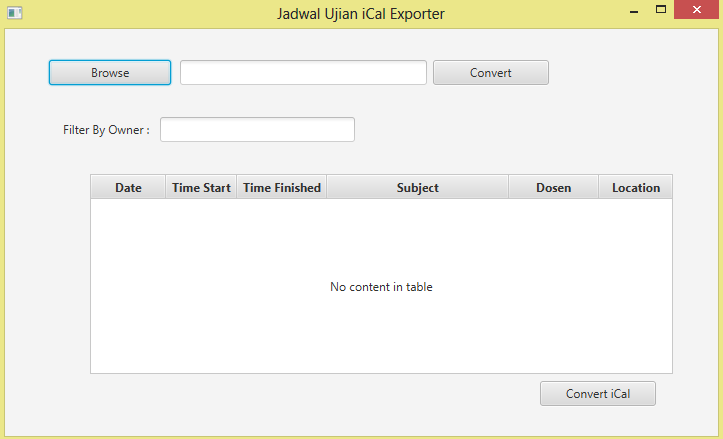
\includegraphics[scale=0.7]{Gambar/implementAntarmuka}
		\caption{Tampilan antarmuka perangkat lunak}
		\label{fig:implementAntarmuka}
		\end{figure}
	\item Tampilan Antarmuka ketika file excel jadwal mengawas telah dimasukan
		\begin{figure}[H]
		\centering
		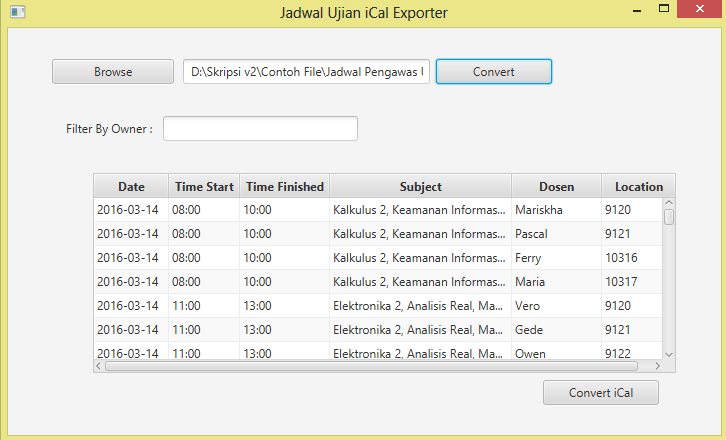
\includegraphics[scale=0.7]{Gambar/implementAntarmuka2}
		\caption{Tampilan antarmuka setelah file mengawas dimasukan}
		\label{fig:implementAntarmuka}
		\end{figure}
\end{enumerate}

\section{Pengujian}
Pada subbab ini akan dilakukan pengujian pada perangkat lunak untuk mengetahui apakah program dapat berjalan sesuai dengan apa yang di inginkan. Terdapat dua pengujian yaitu :
\begin{enumerate}
	\item Pengujian Fungsional.
	\item Pengujian Eksperimental.
\end{enumerate}

\subsection{Pengujian Fungsional}
Pada pengujian ini akan di uji mengenai fungsionalitas dari perangkat lunak ini, Berikut hasil pengujiannya : 
\begin{table}[H]
	\centering
		\caption{Tabel hasil pengujian fungsional}
		\label{tab:fungsional}
		\begin{tabular}{ | p{4cm} | p{4cm} | p{4cm} | c |}
			\hline
				Hal yang diuji & Hasil yang diharapkan & Hasil Pengujian & Status \\ \hline
				Browse file Excel & PL dapat melakukan browse file excel & PL dapat melakukan browse file excel & OK \\ \hline
				Path File Excel & PL dapat menangkap path file dari input & PL dapat menangkap path file dari input & OK \\ \hline
				Menampilkan Jadwal ke layar & PL menampilkan ke layar file excel yang telah dibaca  & PL menampilkan ke layar file excel yang telah dibaca & OK \\ \hline
				Konversi ke iCal & PL dapat mengkonversi jadwal kedalam iCalendar & PL dapat mengkonversi jadwal kedalam iCalendar & OK \\ \hline
				Filter nama dosen & PL dapat menampilkan nama dosen yang telah di filter & PL dapat menampilkan nama dosen yang telah di filter & OK \\ \hline
				Hasil Filter dapat dikonversi ke iCal & Hasil Filter pada PL dapat di konversikan kedalam iCal & Hasil Filter pada PL dapat di konversikan kedalam iCal & OK \\ \hline
				Import Google Calendar & Hasil konversi PL dapat di masukan kedalam Google Calendar & Hasil konversi PL dapat di masukan kedalam Google Calendar & OK \\ \hline
				Dapat dibuka di Outlook & Hasil konversi PL dapat di buka di Outlook & Hasil konversi PL dapat di buka di Outlook & OK \\ \hline
				Hasil filter dapat di import Google Calendar & Hasil filter konversi PL dapat di masukan kedalam Google Calendar & Hasil filter konversi PL dapat di masukan kedalam Google Calendar & OK \\ \hline
				Hasil filter Dapat dibuka di Outlook & Hasil filter konversi PL dapat di buka di Outlook & Hasil filter konversi PL dapat di buka di Outlook & OK \\ \hline
		\end{tabular}
\end{table}

Berikut ini adalah tampilan dari hasil pengujian yang telah dilakukan pada tabel ~\ref{tab:fungsional} :
\begin{enumerate}
	\item Browse File
		\begin{figure}[H]
		\centering
		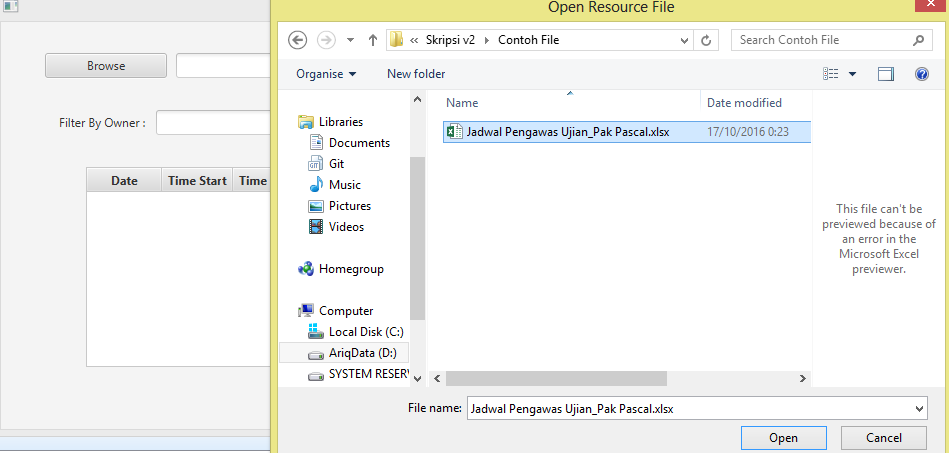
\includegraphics[scale=0.7]{Gambar/browseFile}
		\caption{Tampilan browse file excel mengawas ujian}
		\label{fig:browseFile}
		\end{figure}
	\item Path File Excel
		\begin{figure}[H]
		\centering
		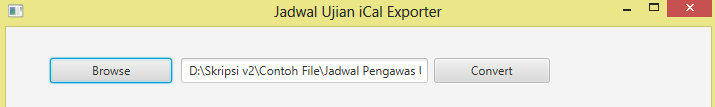
\includegraphics[scale=0.7]{Gambar/pathFile}
		\caption{Tampilan path file excel mengawas ujian}
		\label{fig:pathFile}
		\end{figure}
	\item Menampilkan jadwal ke layar
		\begin{figure}[H]
		\centering
		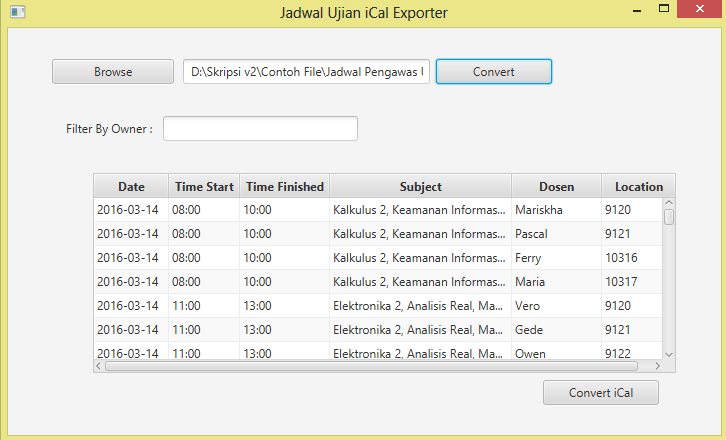
\includegraphics[scale=0.7]{Gambar/implementAntarmuka2}
		\caption{PL menampilkan jadwal ke layar}
		\label{fig:jadwalKeLayar}
		\end{figure}
	\item Konversi ke iCal
		\begin{figure}[H]
		\centering
		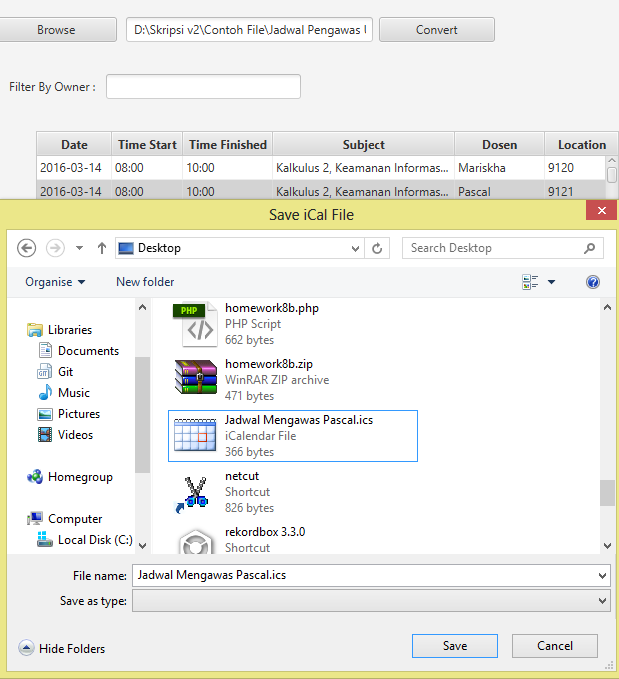
\includegraphics[scale=0.5]{Gambar/konversiiCal}
		\caption{PL mengkonversi jadwal ke format iCal}
		\label{fig:konversiiCal}
		\end{figure}
		
		\begin{figure}[H]
		\centering
		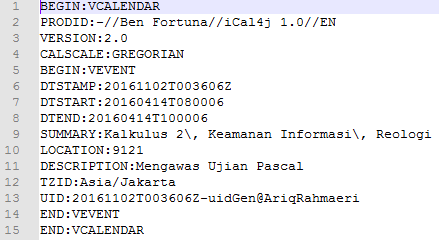
\includegraphics[scale=0.7]{Gambar/fileiCal}
		\caption{File iCal}
		\label{fig:fileiCal}
		\end{figure}
	\item Filter nama dosen
		\begin{figure}[H]
		\centering
		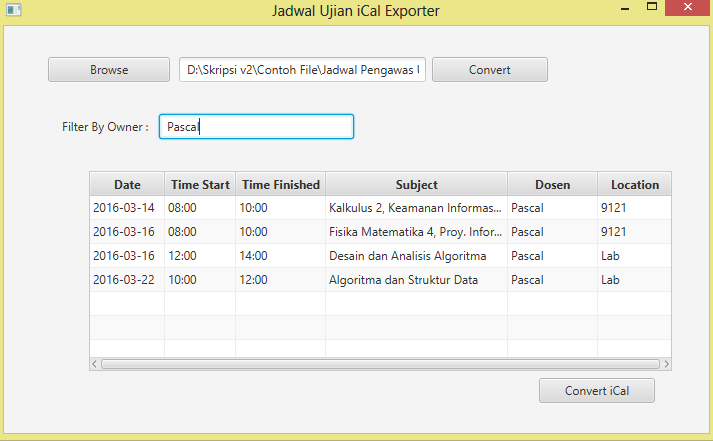
\includegraphics[scale=0.7]{Gambar/filterDosen}
		\caption{Hasil pengujian filter nama dosen}
		\label{fig:filterDosen}
		\end{figure}
	\item Convert hasil filter kedalam iCal
		\begin{figure}[H]
		\centering
		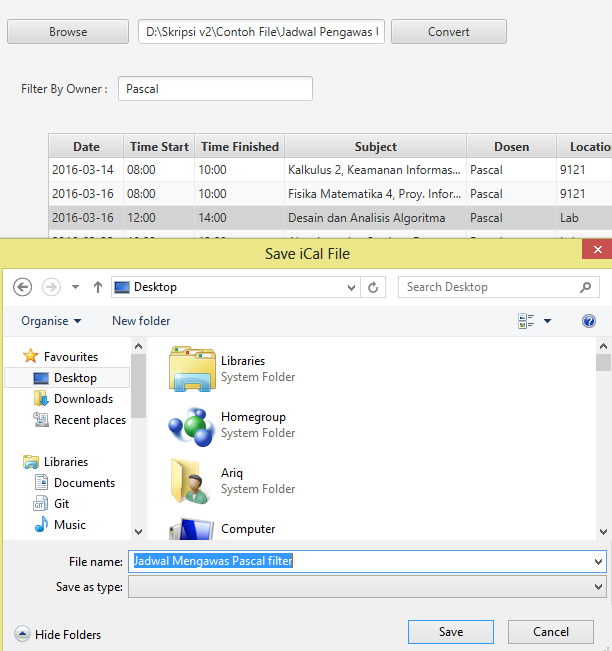
\includegraphics[scale=0.5]{Gambar/filterKonvertiCal}
		\caption{Hasil pengujian convert hasil filter kedalam iCal}
		\label{fig:filterKonvertiCal}
		\end{figure}
		
		\begin{figure}[H]
		\centering
		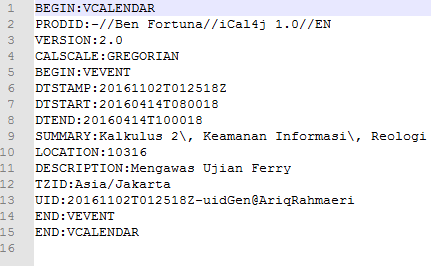
\includegraphics[scale=0.5]{Gambar/fileiCalFilter}
		\caption{File iCal Filter}
		\label{fig:fileiCalFilter}
		\end{figure}
	
	\item Import Google Calendar
		\begin{figure}[H]
		\centering
		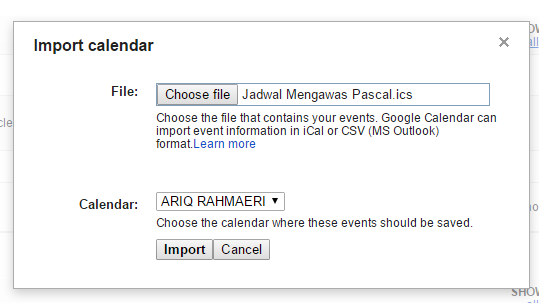
\includegraphics[scale=0.7]{Gambar/importGC}
		\caption{Hasil pengujian import kedalam Google Calendar}
		\label{fig:importGC}
		\end{figure}
		
		\begin{figure}[H]
		\centering
		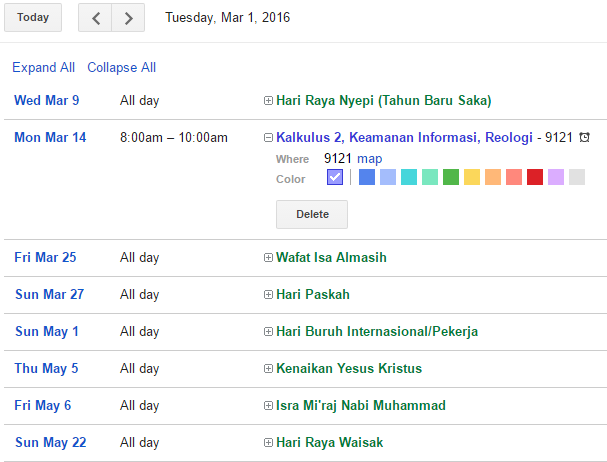
\includegraphics[scale=0.7]{Gambar/hasilGC}
		\caption{Hasil import ke Google Calendar}
		\label{fig:hasilGC}
		\end{figure}
		
		\begin{figure}[H]
		\centering
		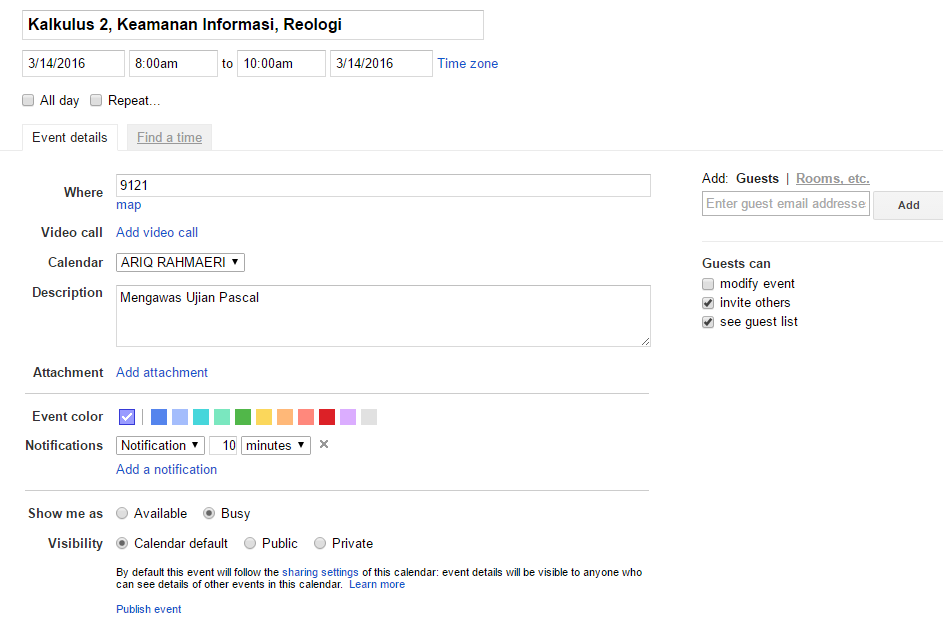
\includegraphics[scale=0.5]{Gambar/hasilGC2}
		\caption{Hasil import ke Google Calendar bagian 2 }
		\label{fig:hasilGC2}
		\end{figure}
		
		\item Buka di MS Outlook
			\begin{figure}[H]
			\centering
			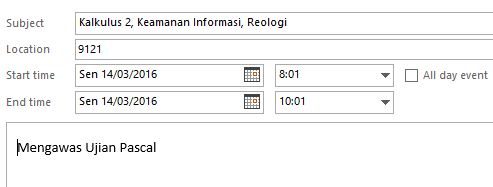
\includegraphics[scale=0.7]{Gambar/hasilOutlook}
			\caption{File hasil Konversi dapat dibuka di MS Outlook }
			\label{fig:hasilOutlook}
			\end{figure}
		
		\item Import hasil filter kedalam Google Calendar
			\begin{figure}[H]
			\centering
			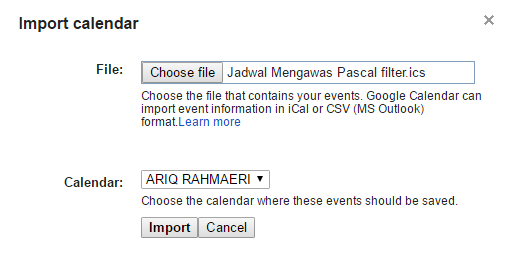
\includegraphics[scale=0.7]{Gambar/importGCFilter}
			\caption{Hasil pengujian import file yang di filter kedalam Google Calendar }
			\label{fig:importGCFilter}
			\end{figure}
			
			\begin{figure}[H]
			\centering
			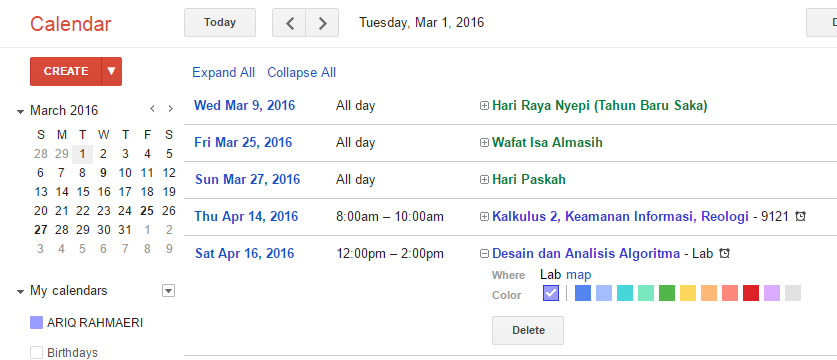
\includegraphics[scale=0.7]{Gambar/hasilGCFilter}
			\caption{Hasil import file yang di filter ke Google Calendar}
			\label{fig:hasilGCFilter}
			\end{figure}
			
			\begin{figure}[H]
			\centering
			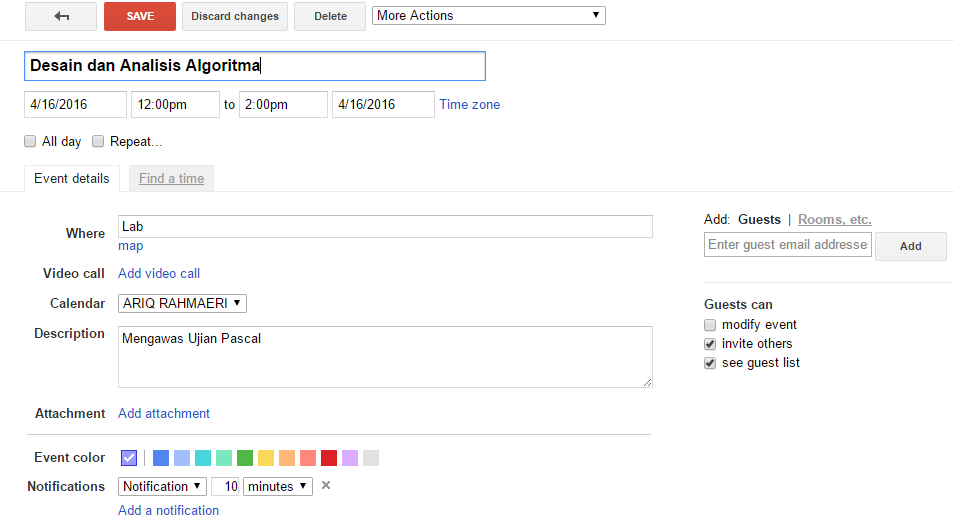
\includegraphics[scale=0.5]{Gambar/hasilGCFilter2}
			\caption{Hasil import file yang di filter ke Google Calendar bagian 2 }
			\label{fig:hasilGCFilter2}
			\end{figure}
			
		\item Buka hasil filter di MS Outlook
			\begin{figure}[H]
			\centering
			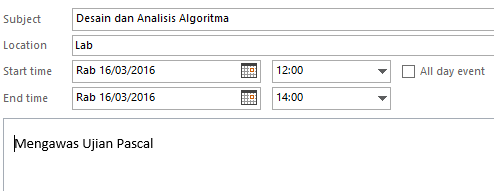
\includegraphics[scale=0.7]{Gambar/hasilOutlookFilter}
			\caption{File hasil filter dapat dibuka di MS Outlook }
			\label{fig:hasilOutlookFilter}
			\end{figure}
			
		
\end{enumerate} 

